%!TEX root = dolgozat.tex
%%%%%%%%%%%%%%%%%%%%%%%%%%%%%%%%%%%%%%%%%%%%%%%%%%%%%%%%%%%%%%%%%%%%%%%
\chapter{Képek előfeldolgozása}\label{ch:PREPROC}
%%%%%%%%%%%%%%%%%%%%%%%%%%%%%%%%%%%%%%%%%%%%%%%%%%%%%%%%%%%%%%%%%%%%%%%

\begin{osszefoglal}
Annak érdekében, hogy egyszerűsítsem a bevitt adatokat, előfeldolgozást végzek a képeken a színük alapján. A neurális háló a pixelek szürke árnyalatával dolgozik. 
A képek különböző fényviszonyok mellett készültek, ennek köszönhetően némelyik nagyon világos, mások pedig nagyon sötétek.

Megjegyzés: A képek valós környezetből származnak, így más objektumokat is tartalmazhatnak, mint például faágak.

\end{osszefoglal}

\section{Színterek}\label{sec:PREPROC:colorSpaces}

A szín a módja annak, ahogyan az emberi látórendszer a bejövő elektromágneses sugárzást értelmezi. Az a tartomány, ahol a rendszer színként érzékeli ezt a sugárzást körülbelül 400 és 830 nm-es hullámhosszak között jelentkezik (személytől függően változhat némileg) \cite{17}. 

A színterek pontosan meghatároznak színeket az érzékelhető hullámhossz tartományból. 
Arra szolgálnak, hogy könnyebben tudjuk meghatározni, létrehozni és felfogni a színeket. Egy színt általában három paraméter határoz meg. Ezek fejezik ki az adott szín helyét az illető színtérben. Különböző színtereket ismerünk, attól függően válasszuk ki a megfelelőt, hogy mire akarjuk alkalmazni \cite{4}. 






\subsection{RGB színtér}\label{sec:PREPROC:rgb}

Az RGB színtér (\ref{fig:RGBColorSpace}) egy additív színrendszer, mely a tri-kromatikus elméleten alapszik. A tri-kromatikus elmélet lényege, hogy 3 különböző szín segítségével bármilyen szín kikeverhető.  
Az RGB színtér könnyen implementálható, de nem párhuzamos az emberi látással. Az RGB színteret gyakran felhasználják számítógépes alkalmazásokhoz, mert nincs szükség transzformációra ahhoz, hogy megjelenítsük az információt. A színtér legegyszerűbb ábrázolása egy kocka, ahol a 3 tengely a piros, zöld és kék színekkel egyenértékű. 


\subsection{HSV színtér}\label{sec:PREPROC:hsv}

Ellentétben az RGB ábrázolással, a HSV színtér (\ref{fig:HSVColorSpace}) henger-koordinátákat alkalmaz. Ez az egyik leggyakoribb ábrázolási módszer. Az árnyalat(hue) az az emberi érzet, amely szerint egy szín egy másik színre vagy több szín keverékére hasonlít a piros, sárga, zöld és kék színek közül. A szín telítettsége (saturation) egy szín színessége és a fényessége közti arány. A fényesség (value-brightness) az az emberi érzet, hogy egy terület több vagy kevesebb fényt áraszt magából. 


\begin{figure}[h]
\centering

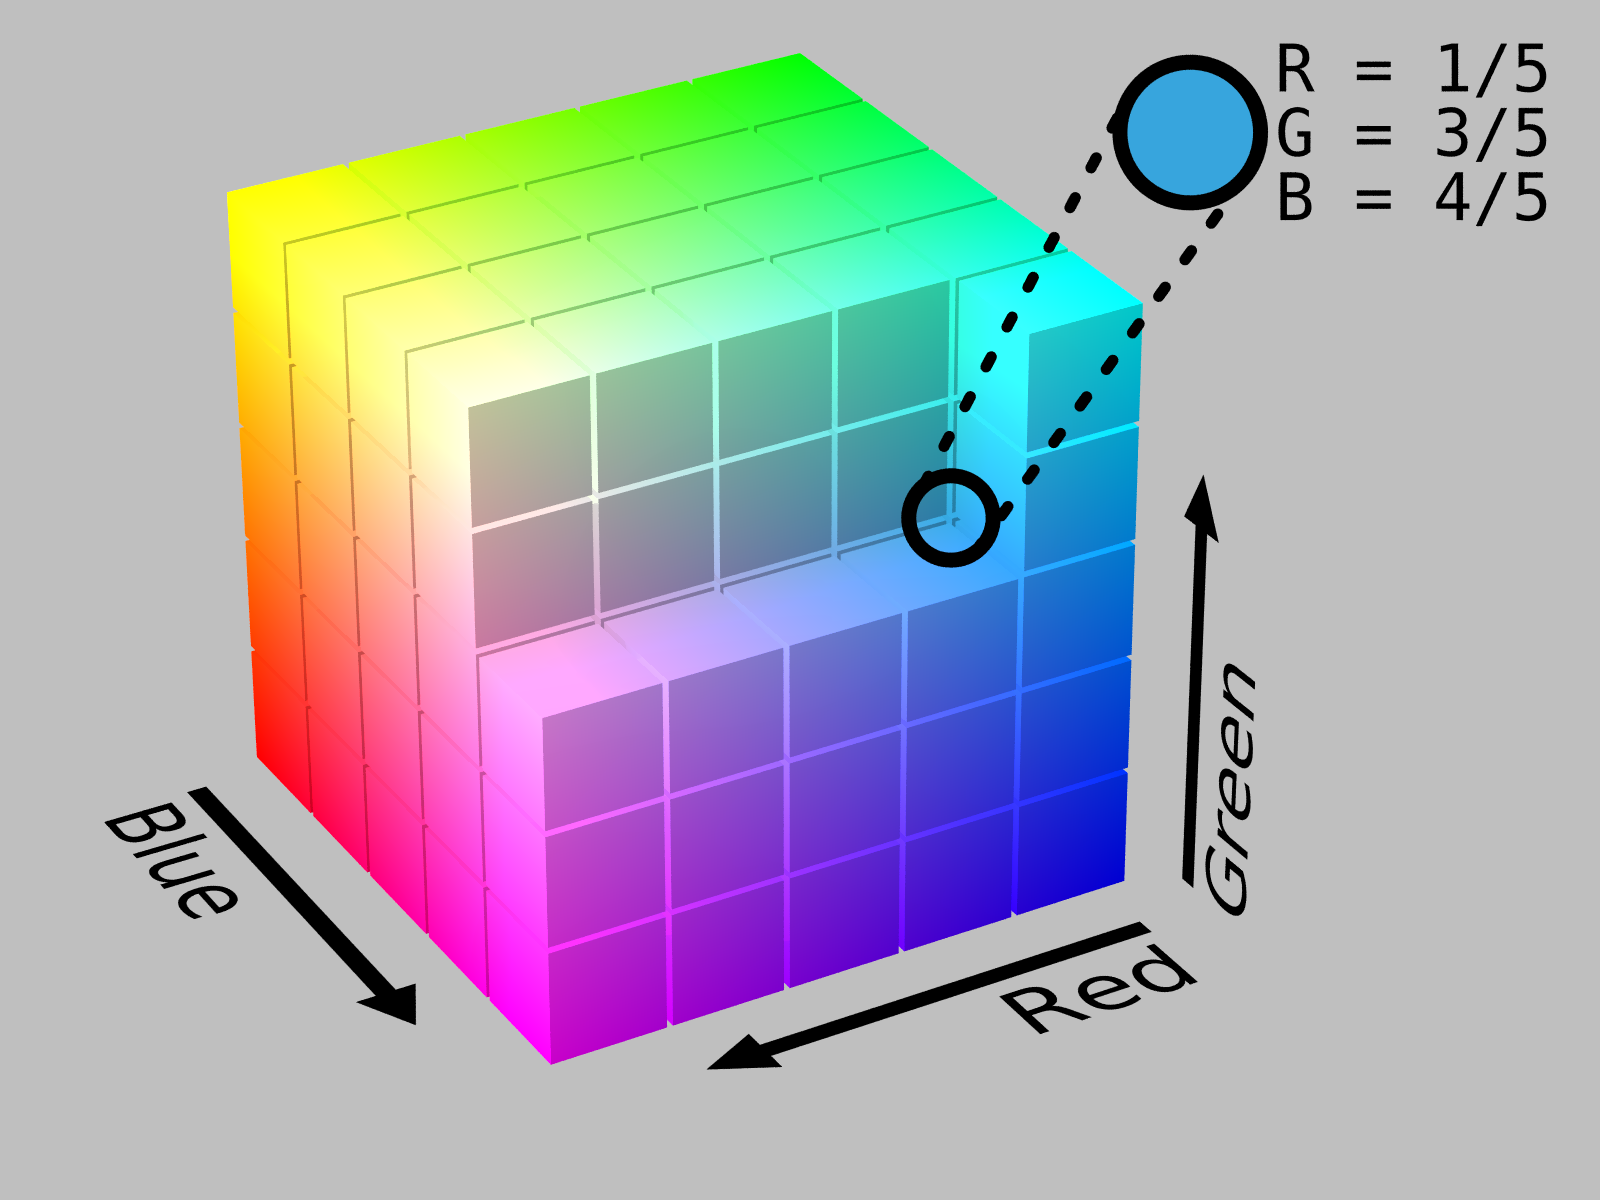
\includegraphics[scale=0.1]{RGBColorSpace}
\caption{RGB színtér}
\small forrás:\url{http://upload.wikimedia.org/wikipedia/commons/8/83/RGB_Cube_Show_lowgamma_cutout_b.png}
\label{fig:RGBColorSpace}
\end{figure}

\begin{figure}[h]
\centering

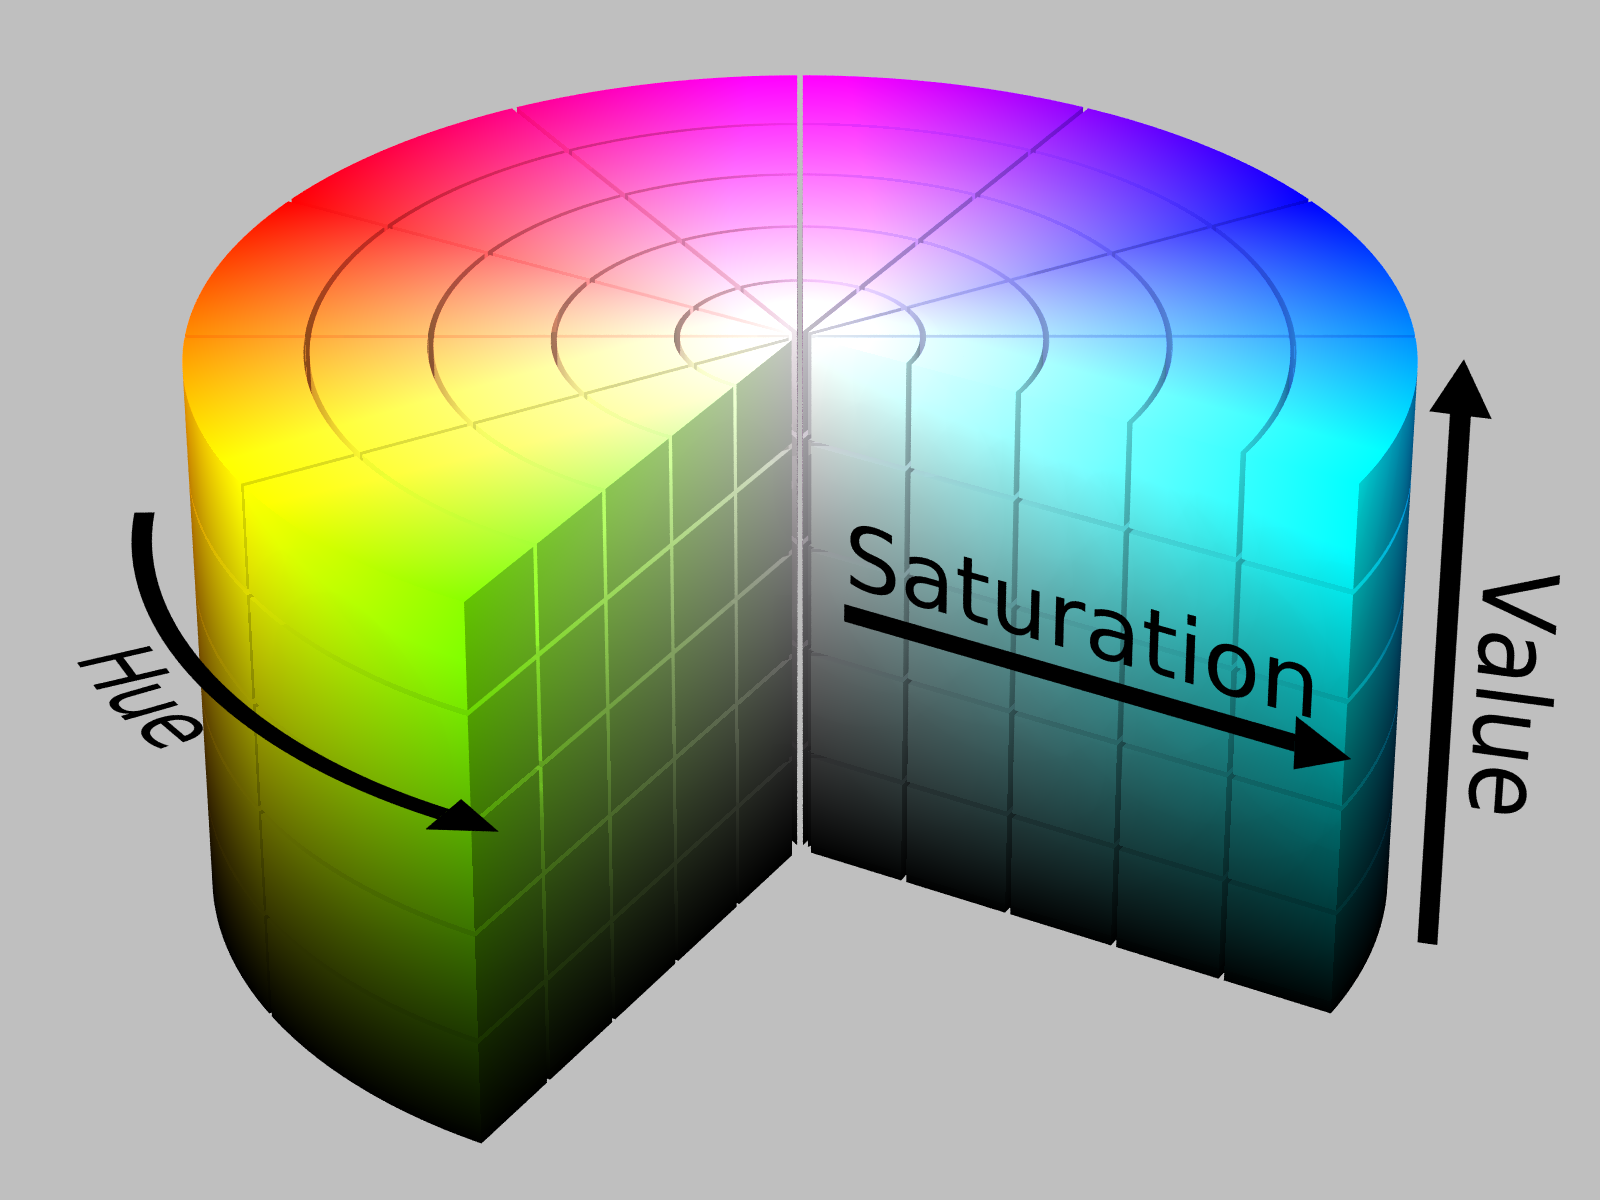
\includegraphics[scale=0.1]{HSVColorSpace}
\caption{HSV színtér}
\small forrás:\url{http://upload.wikimedia.org/wikipedia/commons/0/0d/HSV_color_solid_cylinder_alpha_lowgamma.png}
\label{fig:HSVColorSpace}
\end{figure}

\section{Megvalósítás}\label{sec:PREPROC:implement}

A forgalmi táblák figyelemfelkeltőek kell legyenek, ezért jól látható színeket használnak, mint például piros, kék, sárga, fekete és fehér.

A bemeneti képeket szín alapján szűröm, ezáltal felépítek egy új, fekete-fehér képet. Ha az árnyalat, a telítettség és a fényesség egy bizonyos intervallumban helyezkedik el, az új kép megfelelő pixelje fekete lesz, különben fehér. Ezeket az intervallumokat kísérletezéssel és a \ref{fig:colorWheel} ábra segítségével határoztam meg.

\begin{figure}[h]

\centering 
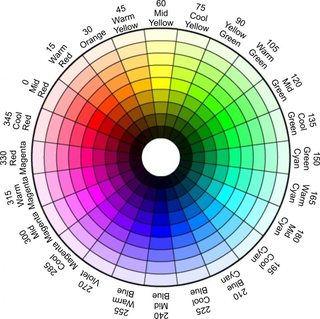
\includegraphics[scale=0.5]{ColorWheel}
\caption{Színkör}
\small forrás:\url{http://stackoverflow.com/questions/21737613/image-of-hsv-color-wheel-for-opencv}
\label{fig:colorWheel} 

\end{figure}

\begin{center}
\begin{table}[h]
\centering
\begin{tabular}{ |p{3cm}||p{3cm}|p{3cm}|p{3cm}|  }
 \hline
 Szín & Árnyalat & Telítettség & Fényesség\\
 \hline
 Piros   & 0-20, 340-360    &>0.3& >0.2\\
 Sárga &   25-60  & >0.3 & >0.2\\
 Kék & 180-270 & >0.3 & >0.2\\
 Fekete    & - & - & <0.3\\
 \hline
\end{tabular}


\caption{Elfogadási tartomány}
\label{table:1}
\end{table}
\end{center}

\section{Átméretezés}

Mivel a tanulási adatok és a teszt adatból kivágott képek mérete is változó, a képeket átméretezem 25x25 pixelre és ezzel dolgozom tovább. Ennek következtében adatvesztés és torzulás léphet fel, amikor más méretű képet méretezek át.
